\section{Podstata simulačních experimentů a jejich průběh}

Cílém experimentů bylo zjistit jak často je chata bez energie a o kolik se tím potenciálně připravujeme zákazníků. Dále jaké jsou možnosti řešení dobu bez energie minimalizovat. Ať už přistavěním dalšího zdroje energie, či zvýšením kapacity akumulátorů.



\subsection{Postup experimentování}

Nejprve simulujeme provoz chaty s údaji které maximálně odrážejí současnost pro několik let běžného provozu. Můžeme se zaměřit pouze na hlavní sezónu, kdy je nápor největší. Hrozí nejvíce výpadků energie a taky mají nejhorší následky, přicházíme o zákazníky. Analyzujeme potenciální ztrátu zákazníků, dobu po kterou jsou akumulátory zaplněné a dobu po kterou jsme bez energie.

Pro další experimentování jsme zvýšili počet větrných turbín a přistavěli další solární panely, střecha chaty není úplně zaplněná.



\subsection{Jednotlivé experimenty}

\subsection{Prvotní experimenty}

Na základě statistik~\ref{tab:res_1} z prvního experimentu jsme zjistili, že náš model dává podivné výsledky při generování energie. Konkrétně, že jediný solární panel generuje daleko více energie než jedna větrná turbína. Pravděpodobně jsme udělali někde chybu při sbírání faktů. Generování energie větrnou turbínou jsme zvýšili.

\begin{figure}[H]
    \begin{verbatim}
    +----------------------------------------------------------+
    | STATISTIC Energy generated by wind turbines              |
    +----------------------------------------------------------+
    |  Min = 0                       Max = 83                  |
    |  Number of records = 210240                              |
    |  Average value = 48.7062                                 |
    |  Standard deviation = 17.6815                            |
    +----------------------------------------------------------+
    +----------------------------------------------------------+
    | STATISTIC Energy generated by solar panels               |
    +----------------------------------------------------------+
    |  Min = 63                      Max = 306                 |
    |  Number of records = 2522880                             |
    |  Average value = 190.573                                 |
    |  Standard deviation = 87.0823                            |
    +----------------------------------------------------------+
    \end{verbatim}
    \caption{Výsledky experimentu 1}
    \label{tab:res_1}
\end{figure}

Na základě statistik~\ref{tab:res_2} z druhého experimentu jsme zjistili, že zákazníci si berou příliš mnoho energie. Pravděpodobně jsme špatně odhadli spotřebu na zákazníka, kterou jsme zakládali na průměrné spotřebě hotelů (viz kapitola ~\ref{chap:analysis}). Spotřebu návštěvníků jsme snížili na 4.5\,kWh pro noc a 1.0\,kWh pro den.

\begin{figure}[H]
    \begin{verbatim}
        +----------------------------------------------------------+
        | STATISTIC Number of guests in the hut at the same time   |
        +----------------------------------------------------------+
        |  Min = 1                       Max = 185                 |
        |  Number of records = 525600                              |
        |  Average value = 54.3021                                 |
        |  Standard deviation = 58.6799                            |
        +----------------------------------------------------------+
        +----------------------------------------------------------+
        | STATISTIC Energy need per visitor                        |
        +----------------------------------------------------------+
        |  Min = 0                       Max = 6369.79             |
        |  Time = 0 - 3.1536e+10                                   |
        |  Number of records = 49404                               |
        |  Average value = 1625.7                                  |
        +----------------------------------------------------------+
        +----------------------------------------------------------+
        | STATISTIC Visitors per day                               |
        +----------------------------------------------------------+
        |  Min = 18                      Max = 414                 |
        |  Number of records = 365                                 |
        |  Average value = 135.353                                 |
        |  Standard deviation = 145.575                            |
        +----------------------------------------------------------+
    \end{verbatim}
    \caption{Výsledky experimentu 2}
    \label{tab:res_2}
\end{figure}


Na základě grafu z obrázku~\ref{fig:graph_1} jsme zjistili, že v půlce hlavní seźony energie dojde a již se ji nepodaří doplňovat. Půlku sezóny tedy bude chata kompletně bez energie. Mimo hlavní sezónu je výdaj výrazně nižší, proto dostupná energie bude téměř stále na maximu.


\begin{figure}[H]
    \centering
    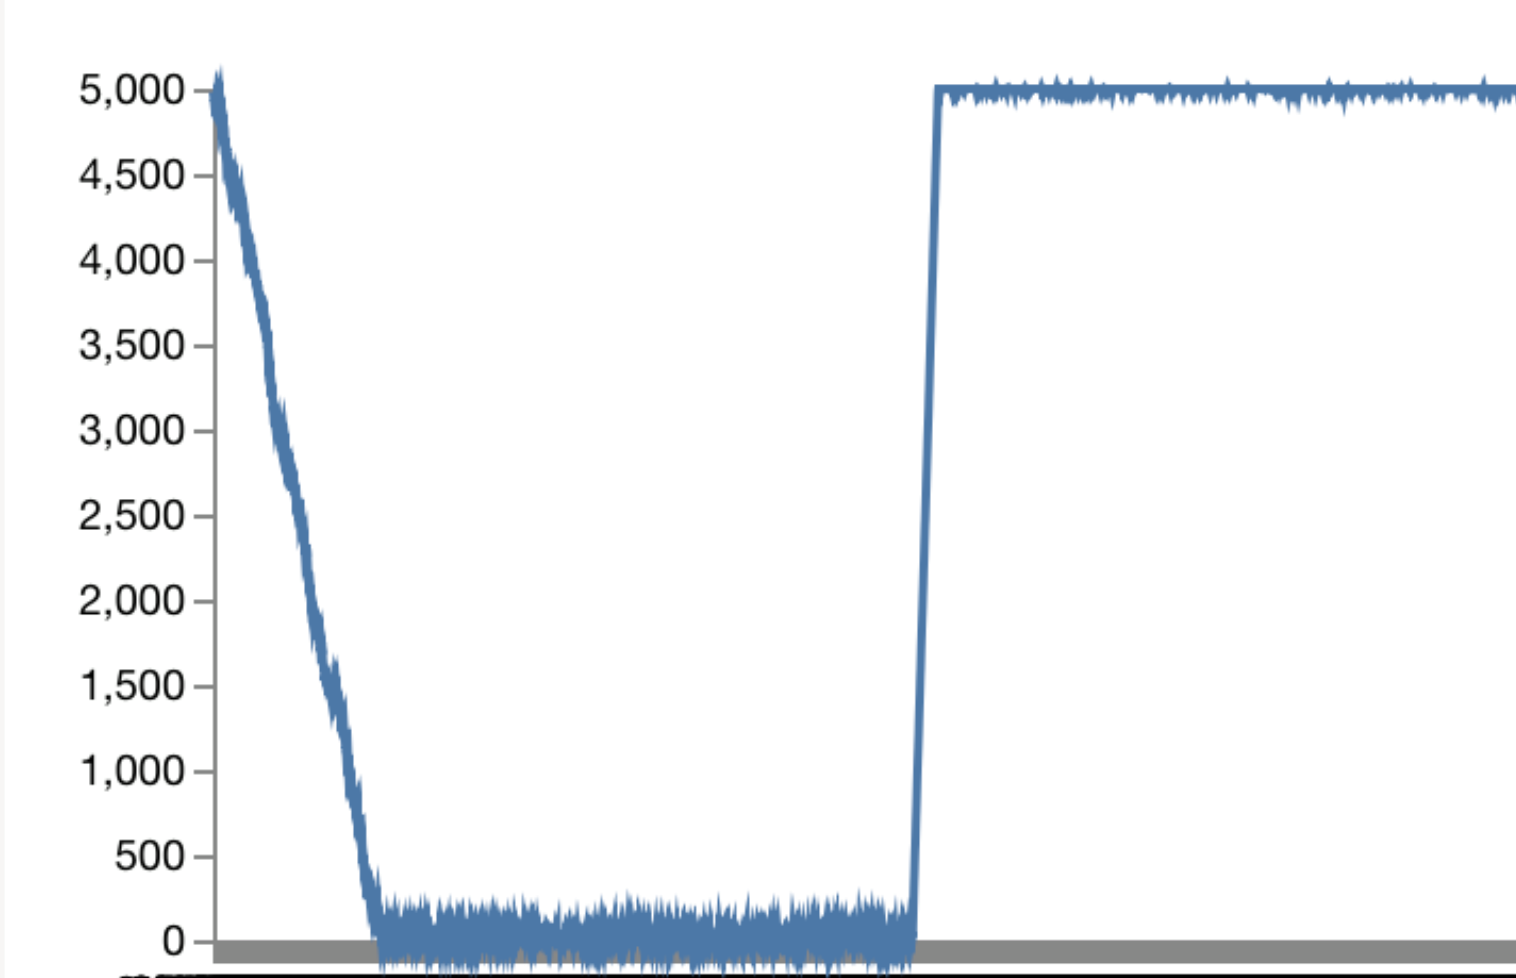
\includegraphics[width=.75\textwidth]{images/graph_1.png}\hfill
    \caption{Množství energie v průběhu roku}
    \label{fig:graph_1}
\end{figure}



\subsubsection{Přidání větrné turbíny}

Stav v případě, že bychom se rozhodli postavit další větrnou turbínu je zachycen na obrázku~\ref{fig:graph_2}. Přistavění větrné turbíny by situaci vyřešilo pouze částěčně.

\begin{figure}[H]
    \centering
    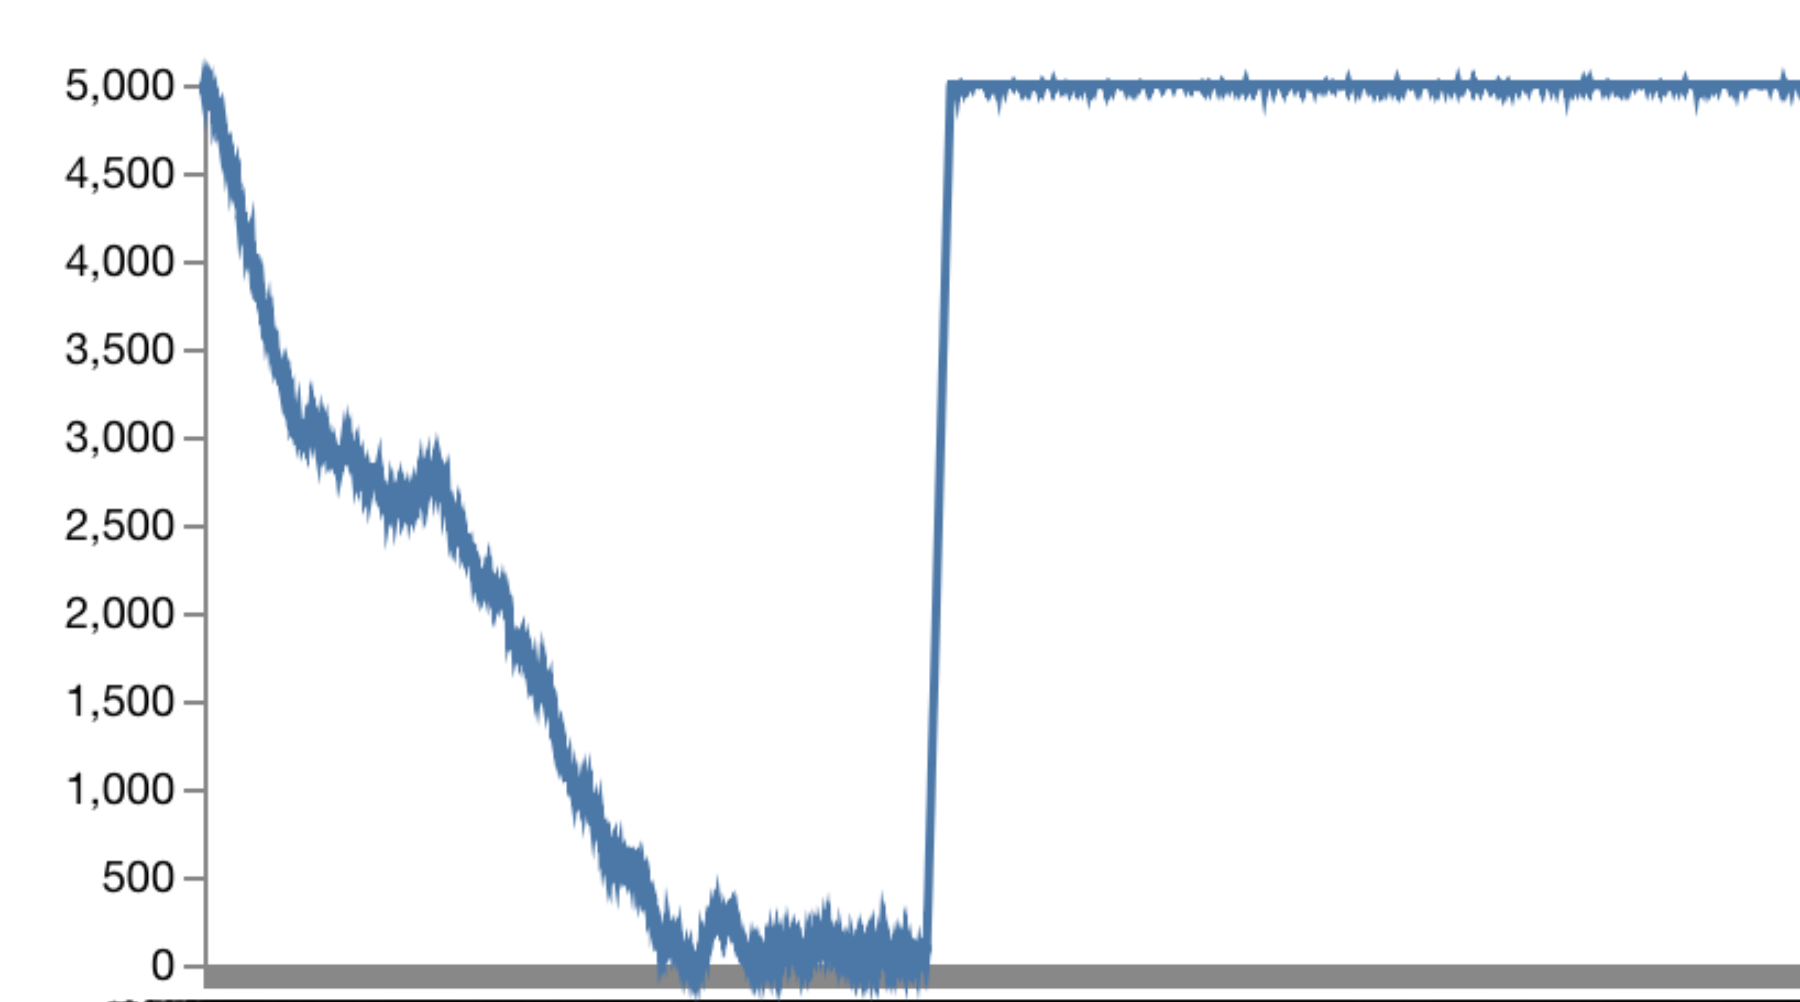
\includegraphics[width=.75\textwidth]{images/graph_2.png}\hfill
    \caption{Množství energie v průběhu roku (+1 turbína)}
    \label{fig:graph_2}
\end{figure}


\subsubsection{Přidání ještě solárních panelů}

Stav v případě, že bychom se rozhodli přidat ještě jeden solární panel je zachycen na obrázku~\ref{fig:graph_3}. Vidíme, že přistavět jeden panel stačí a situace je vyřešena. Chata bude mít stabilně energii po celý rok.

\begin{figure}[H]
    \centering
    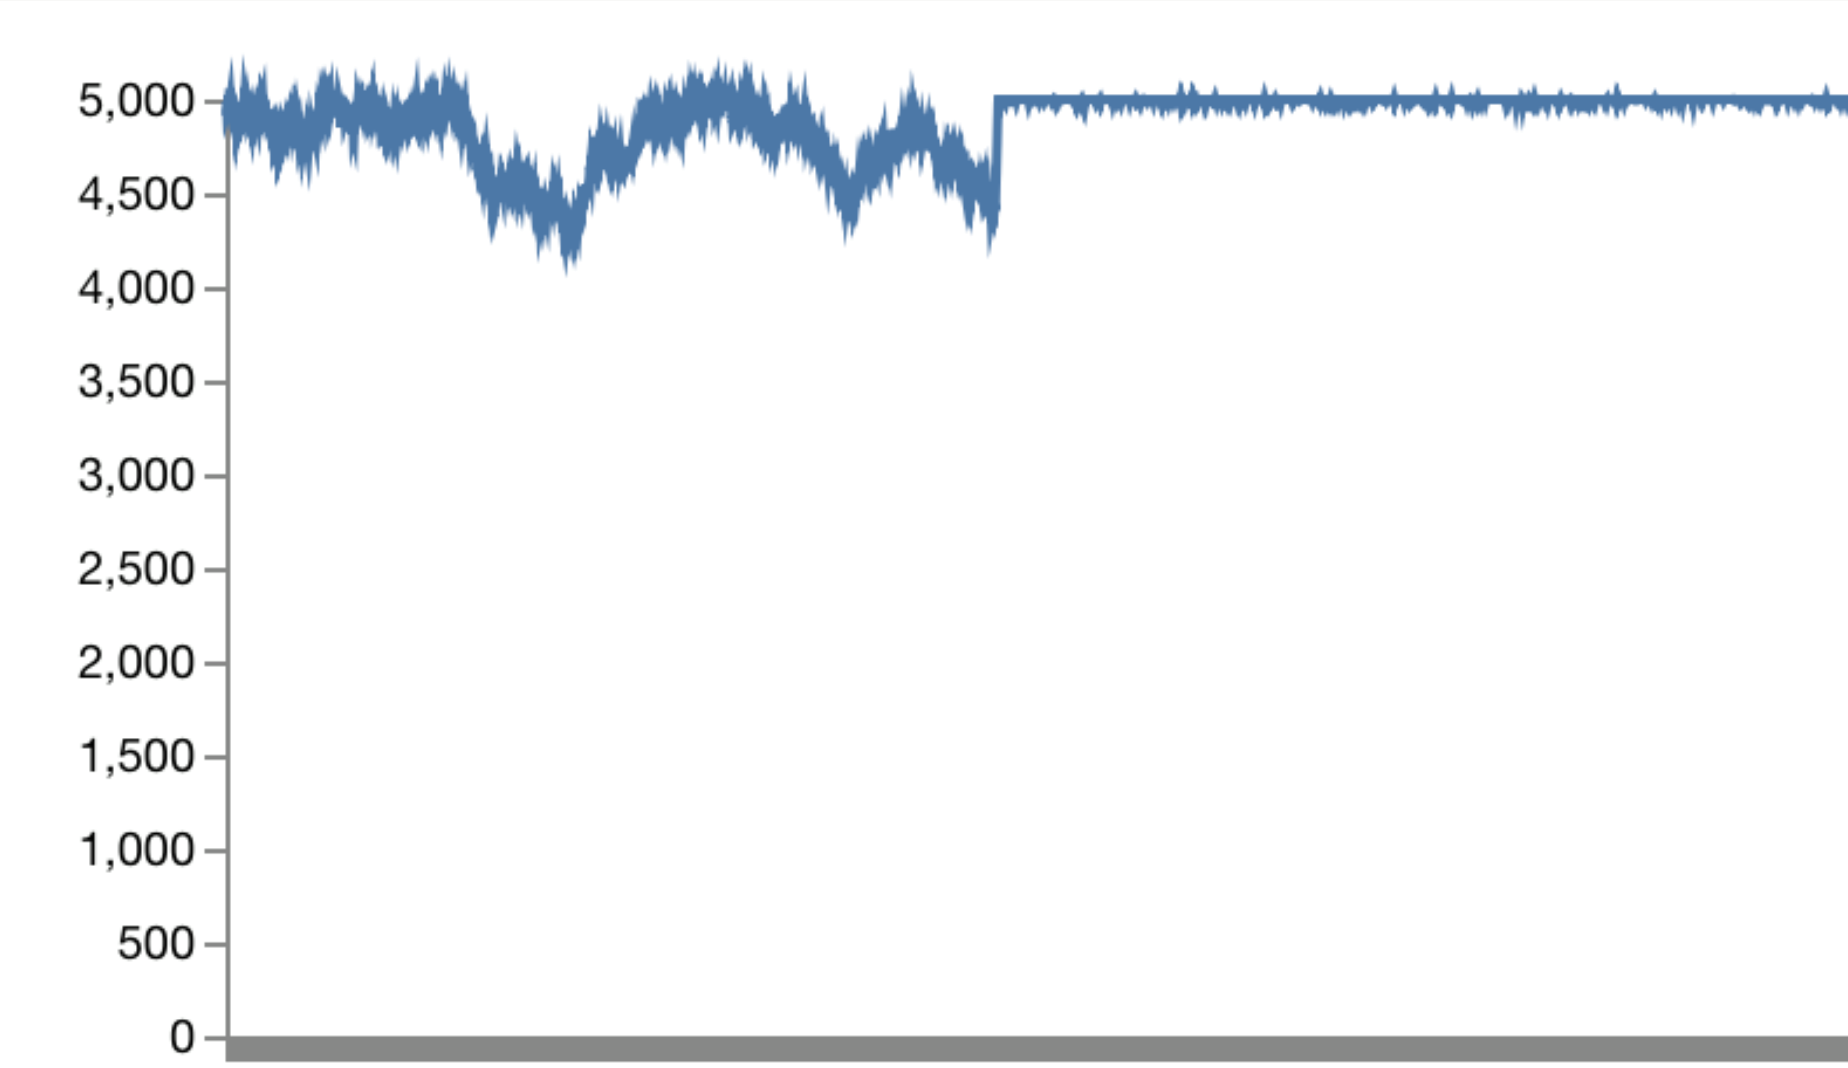
\includegraphics[width=.75\textwidth]{images/graph_3.png}\hfill
    \caption{Množství energie v průběhu roku (+1 turbína a +1 panel)}
    \label{fig:graph_3}
\end{figure}


\subsection{Závěr experimentování}

Z experimentů jsme zjistili, že naše posbíraná data nemusela být naprosto korektní. Někde došlo k nějaké nepřesnosti a nejprve nám vycházeli nesmysli. Postupně jsme upravovali produkci energie větrnou turbínou a spotřebu návštěvníka chaty.

Na dalších experimentech jsme se zjišťovali přidávání zdrojů energie. Ideální případ by byl přistavět jednu větrnou turbínu a jeden solární panel. Již to by stačilo pro zajištění stability energie po celý rok.
